\documentclass[a4paper,10pt]{article}
\usepackage[utf8]{inputenc}
\usepackage{datetime}
\usepackage{listings}
\usepackage{graphicx}
\newdate{date}{17}{02}{2017}
\date{\displaydate{date}}

\title{Homework 1\\Marlen Akimaliev\\BIL622-Numerical Analysis II}
%\author{Share\LaTeX}

\begin{document}

\maketitle

\section{Solve $y'=(x \times y^2+x)/(y-x^2 \times y)$ using Euler method and Runge–Kutta method 4}
\subsection{Solution using Euler method}
Euler’s method for numerically approximating the solution of a first-order initial value problem $y'=f(x,y)$, $y(x_0) = y_0$ as a table of values. To start, we must decide the interval $[x_0 ,x_f]$ that we want to find a solution on, as well as the number of points $n$ that we wish to approximate in that interval. Then taking $h = (x_f-x_0)/(n-1)$ we have $n$ evenly spaced points $x_0, x_1,..., x_n$, with $x_j = x_0+j\times h$. Then our objective is then to fill in the values of $y(x_i)$ in the table below. 
\begin{center}
\begin{tabular}{ |c|c| } 
 \hline
 $x$ & $y$\\
\hline
 $x_0$ & $y_0$ \\ 
 $x_1$ & $y(x_1)$ \\ 
 $x_2$ & $y(x_2)$ \\
 . & . \\
 . & . \\
 . & . \\
 $x_n$ & $y(x_n)$ \\
 \hline
\end{tabular}
\end{center}
Let’s use Euler’s method to approximate the value of the function in the interval [0.0, 0.9] with 10 points. Then $x_0 = 0, y_0 = 1, x_f = 0.9, n = 10$, and $h = (x_f-x_0 )/(n-1)=0.1$. I have the following Python script \cite{euler} to evaluate these values:
\begin{lstlisting}[language=Python]
import numpy as np
from matplotlib import pyplot as plt

def euler( f, x0, y0, x1, n):
	h = (x1-x0)/float(n)              
	t = np.arange(x0, x1+h, h )    
	w = np.zeros((n+1,))
	t[0] = x0
	w[0] = y0   
	for i in range(1,n+1):                       
		w[i] = w[i-1] + h * f(t[i-1], w[i-1])
		t[i] = x0 + i * h
	return t,w
def f(x,y):
	return (x*y**2+x)/(y-x**2*y)
vx,vy = euler(f, 0, 1, 0.9, 10)
for x, y in list(zip(vx, vy))[::1]:
    print("%4.1f %10.16f" % (x, y))
plt.plot(vx, vy, label='approximation' )
plt.title( "Euler's Method Example")
plt.xlabel('Value of x') 
plt.ylabel('Value of y')
plt.legend(loc=4)
plt.grid()
plt.savefig( '1_1.eps', fmt='EPS', dpi=100 )
plt.show()
\end{lstlisting}
I have chosen the interval [0.0, 0.9] because at point $1.0$ value of function will be infinite. Following is the table after filling out the values of $y(x_i)$:
\begin{center}
\begin{tabular}{ |c|c| } 
 \hline
 $x$ & $y$\\
\hline
 $0.0$ & $1.0$ \\ 
 $0.1$ & $1.0202020202020201$ \\ 
 $0.2$ & $1.0618770210354367$ \\
 $0.3$ & $1.1279299548267183$\\
 $0.4$ & $1.223858994411555$\\
 $0.5$ & $1.3599221002436146$\\
 $0.6$ & $1.5563525693735585$\\
 $0.7$ & $1.8581596972015748$\\
 $0.8$ & $2.3906767135460782$\\
 $0.9$ & $3.7212406540001011$\\
 \hline
\end{tabular}
\end{center}
If we try to plot the graph of this function result will be as follows:
\begin{figure}[h]
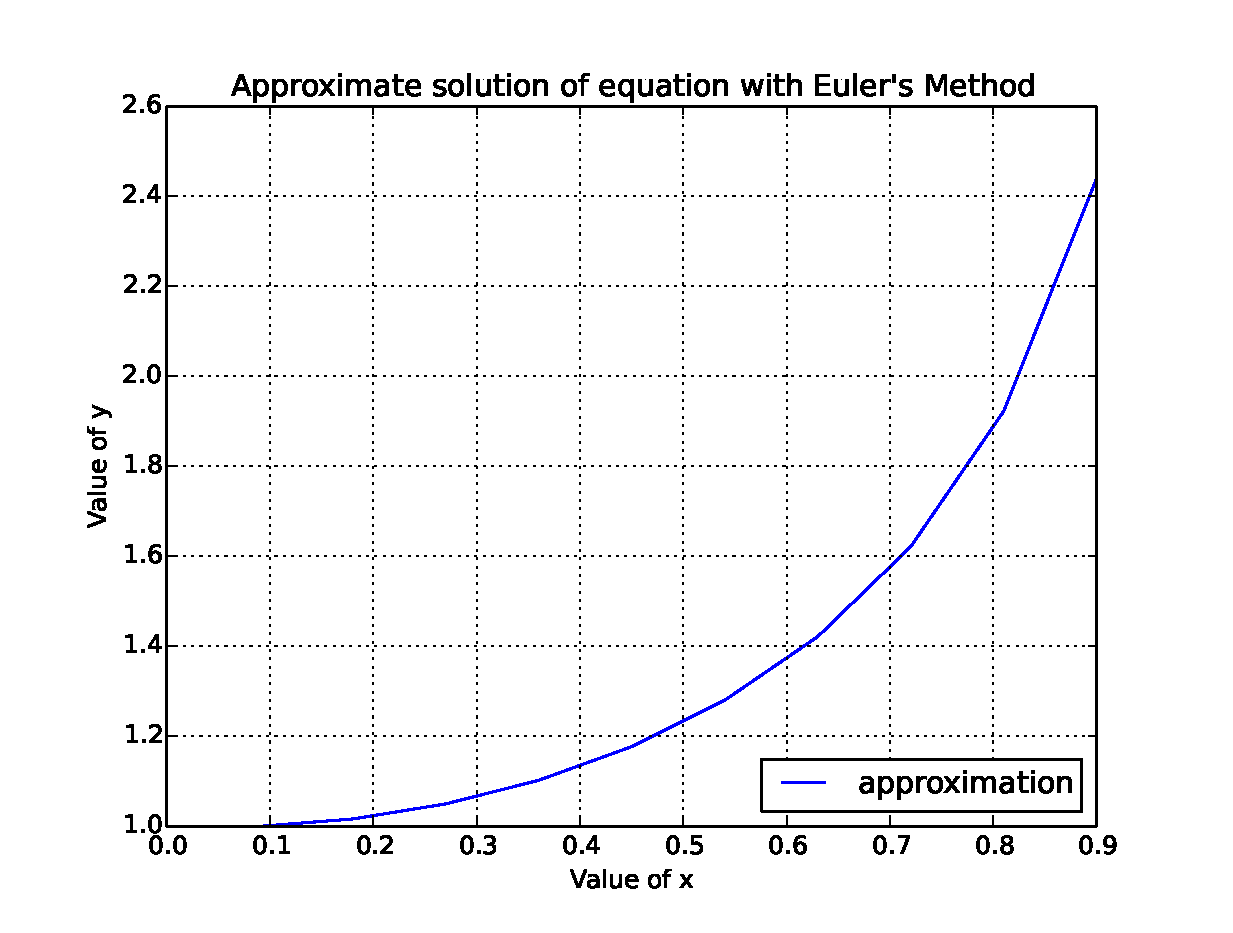
\includegraphics[width=8cm]{1.eps}
\end{figure}
\subsection{Solution using Runge-Kutta method 4}
Runge-Kutta 4 method is stated as follows: Starting with a given $y_n$ and $x_n$ calculate:\\
$k_1= h \times y'(x_n, y_n)$\\
$k_2= h \times y'(x_n, + 1/2 \times h, y_n + 1/2 \times k_1)$\\
$k_3= h \times y'(x_n, + 1/2 \times h, y_n + 1/2 \times k_2)$\\
$k_4= h \times y'(x_n, + h, y_n + k_3)$\\
then:\\
$y_{n+1}=y_n+1/6 \times (k_1 + 2 \times k_2 + 2\times k_3 + k_4)$\\
$x_{n+1}=x_n+h$

Let’s approximate the value of the function in the interval [0.0, 0.9] with 10 points as it was with Euler's method. Then $x_0 = 0, y_0 = 1, x_f = 0.9, n = 10$, and $h = (x_f-x_0 )/(n-1)=0.1$. I have the following Python script \cite{rosettacode} to evaluate these values:
\begin{lstlisting}[language=Python]
from math import sqrt
from matplotlib import pyplot as plt
 
def rk4(f, x0, y0, x1, n):
    vx = [0] * (n + 1)
    vy = [0] * (n + 1)
    h = (x1 - x0) / float(n)
    vx[0] = x = x0
    vy[0] = y = y0
    for i in range(1, n + 1):
        k1 = h * f(x, y)
        k2 = h * f(x + 0.5 * h, y + 0.5 * k1)
        k3 = h * f(x + 0.5 * h, y + 0.5 * k2)
        k4 = h * f(x + h, y + k3)
        vx[i] = x = x0 + i * h
        vy[i] = y = y + (k1 + k2 + k2 + k3 + k3 + k4) / 6
    return vx, vy
 
def f(x, y):
    return (x*y*y+x)/(y-x*x*y)

vx, vy = rk4(f, 0, 1, 0.9, 10)
for x, y in list(zip(vx, vy))[::1]:
    print("%4.1f %10.16f" % (x, y))

vx2, vy2 = rk4(f, 0, 1, 0.9, 100)
plt.plot(vx2,vy2,'o')
plt.xlabel("Value of x")
plt.ylabel("Value of y")
plt.title("Approximate solution of with Runge-Kutta 4 method")
plt.show()
\end{lstlisting}
Following is the table after filling out the values of $y(x_i)$:
\begin{center}
\begin{tabular}{ |c|c| } 
 \hline
 $x$ & $y$\\
\hline
 $0.0$ & $1.0$ \\ 
 $0.1$ & $1.0081331169094654$ \\ 
 $0.2$ & $1.0329425001919301$ \\
 $0.3$ & $1.0757627926056470$\\
 $0.4$ & $1.223858994411555$\\
 $0.5$ & $1.3502868471569234$\\
 $0.6$ & $1.5219160643979874$\\
 $0.7$ & $1.7756474787541259$\\
 $0.8$ & $2.1945860424968737$\\
 $0.9$ & $3.0879623126444544$\\
 \hline
\end{tabular}
\end{center}
If we try to plot the graph of this function result will be as follows:
\begin{figure}[h]
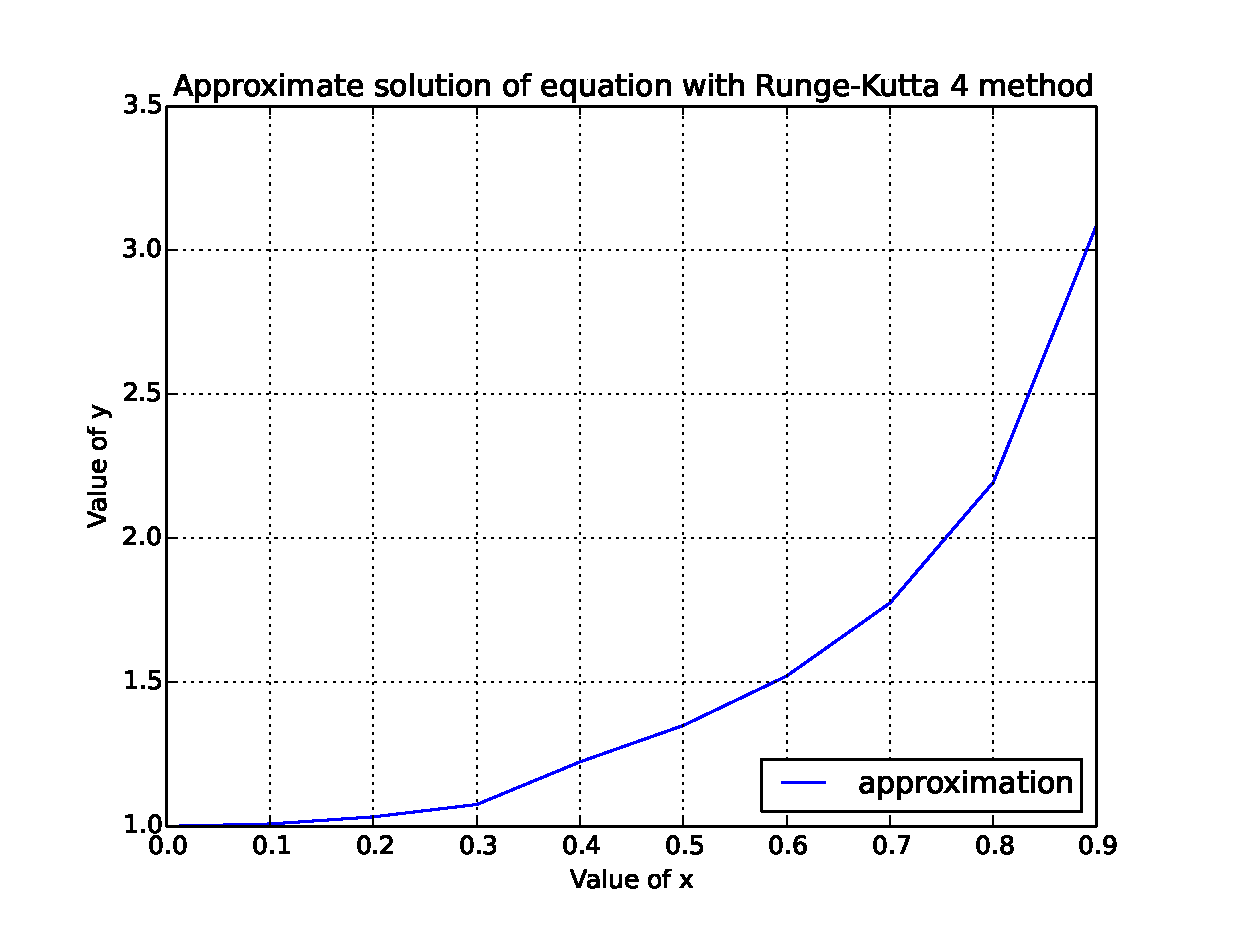
\includegraphics[width=8cm]{2.eps}
\end{figure}
\section{Solve $y'=(1-2*x)/y^2$ using Modified Euler method 1 and Runge-Kutta method 3}
\subsection{Solution using Modified Euler method 1}
Modified Euler method 1 is stated as follows:\\
$y_{i+1} = y_i+h/2(y'_i+y'_{i+1})$\\
$=y_i+h/2(f(x_i,y_i)+f(x_{i+1}, y_{i+1}))$

Let’s approximate the value of the function in the interval [0.0, 1.0] with 10 points. Then $x_0 = 0, y_0 = 1, x_f = 1.0, n = 10$, and $h = (x_f-x_0 )/(n-1)=0.1$. I have the following Python script \cite{connor} to evaluate these values:
\begin{lstlisting}[language=Python]
import numpy as np
from matplotlib import pyplot as plt

def mod_euler( f, x0, y0, x1, n):
	h = (x1-x0)/float(n)
	t = np.arange(x0, x1+h, h )
	w = np.zeros((n+1,))
	t[0] = x0
	w[0] = y0
	for i in range(1,n+1):
		f1 = f( t[i-1], w[i-1] )
		f2 = f( t[i], w[i-1] + h * f1 )
		w[i] = w[i-1] + h * ( f1 + f2 ) / 2.0
		t[i] = x0 + i * h
	return t,w
def f(x,y):
	return (1-2*x)/y**2
vx,vy = mod_euler(f, 0, 1, 1.0, 10)
plt.plot(vx, vy, label='approximation' )
plt.title( "Approximate solution of equation with Modified Euler method 1")
plt.xlabel('Value of x') 
plt.ylabel('Value of y')
plt.legend(loc=4)
plt.grid()
plt.show()
\end{lstlisting}
Following is the table after filling out the values of $y(x_i)$:
\begin{center}
\begin{tabular}{ |c|c| } 
 \hline
 $x$ & $y$\\
\hline
 $0.0$ & $1.0$ \\ 
 $0.1$ & $1.0830578512396694$ \\ 
 $0.2$ & $1.1397927856631667$ \\
 $0.3$ & $1.1771044659164211$\\
 $0.4$ & $1.1984147285629976$\\
 $0.5$ & $1.2053775574789269$\\
 $0.6$ & $1.1984949373933313$\\
 $0.7$ & $1.1772799940498253$\\
 $0.8$ & $1.1401030742252725$\\
 $0.9$ & $1.0835983072329833$\\
 $1.0$ & $1.0010435760606788$ \\
 \hline
\end{tabular}
\end{center}
If we try to plot the graph of this function result will be as follows:
\begin{figure}[h]
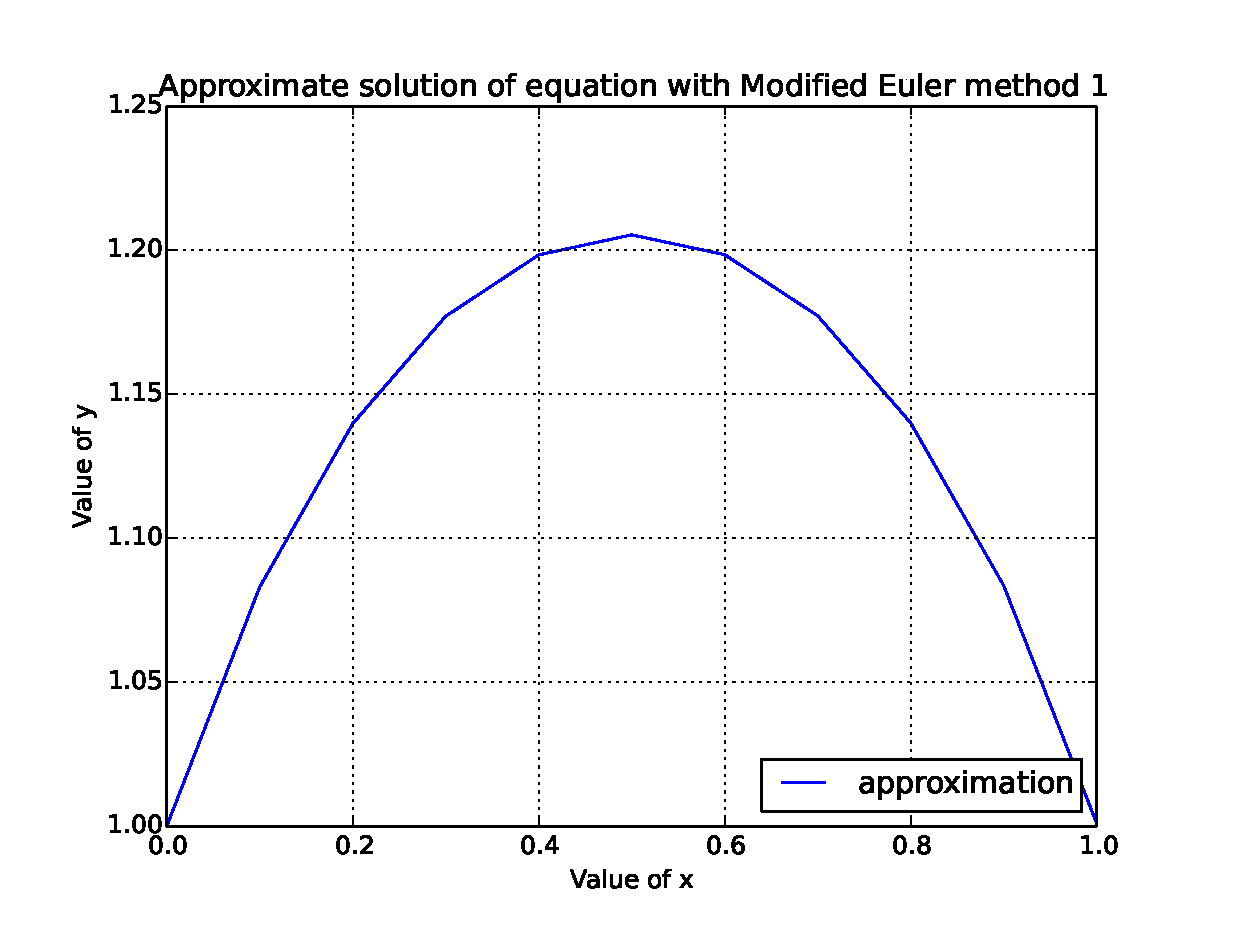
\includegraphics[width=8cm]{2_1.eps}
\end{figure}
\subsection{Solution using Runge-Kutta method 3}
Runge-Kutta 3 method is stated as follows: Starting with a given $y_n$ and $x_n$ calculate:\\
$k_1 = h \times f(x_n, y_n)$\\
$k_2 = h \times f(x_n + h/2, y_n + k_1/2)$\\
$k_3 = h \times f(x_n + h, y_n - k_1 + 2 \times k_2)$\\
then:\\
$y_{n+1}=y_n+1/6 \times (k_1+4\times k_2+k_3)$\\
$x_{n+1}=x_n+h$\\
Let’s approximate the value of the function in the interval [0.0, 1.0] with 10 points. Then $x_0 = 0, y_0 = 1, x_f = 1.0, n = 10$, and $h = (x_f-x_0 )/(n-1)=0.1$. I have modified Python script \cite{rosettacode} to evaluate the values to get the following table of values:
\begin{center}
\begin{tabular}{ |c|c| } 
 \hline
 $x$ & $y$\\
\hline
 $0.0$ & $1.0$ \\ 
 $0.1$ & $1.0828822813050640$ \\ 
 $0.2$ & $1.1395306642445624$ \\
 $0.3$ & $1.1767842783825406$\\
 $0.4$ & $1.1980457654770715$\\
 $0.5$ & $1.2049593292333054$\\
 $0.6$ & $1.1980185265294063$\\
 $0.7$ & $1.1767247315617080$\\
 $0.8$ & $1.1394256727804197$\\
 $0.9$ & $1.0827006273059878$\\
 $1.0$ & $0.9996565522637323$ \\
 \hline
\end{tabular}
\end{center}
If we try to plot the graph of this function result will be as follows:
\begin{figure}[h]
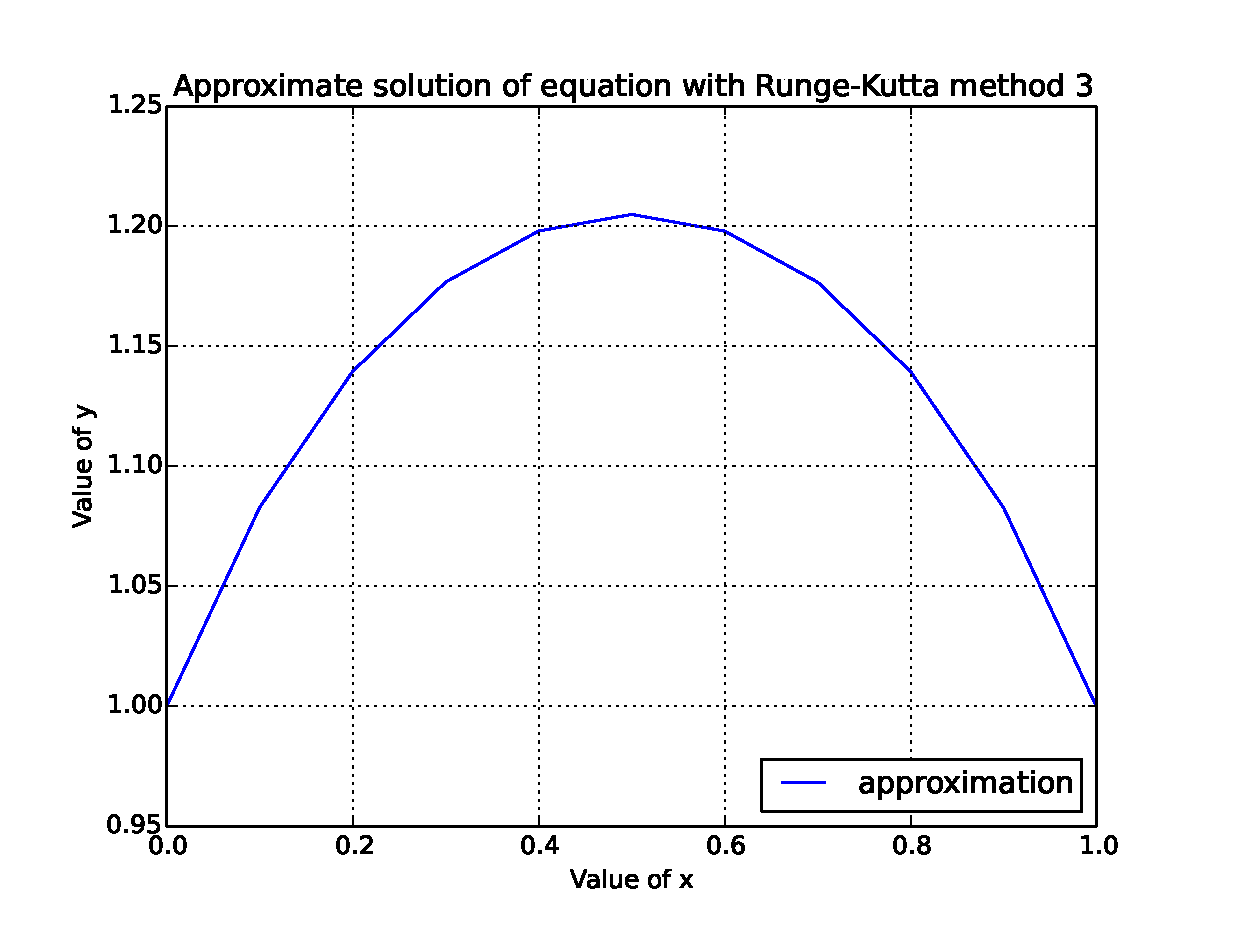
\includegraphics[width=8cm]{2_2.eps}
\end{figure}
\section{Solve $y'=e^{x}-1$ using Modified Euler method 2 and Runge-Kutta method 4}
\subsection{Solution using Runge-Kutta method 4}
Let’s approximate the value of the function in the interval [0.0, 1.0] with 10 points. Then $x_0 = 0, y_0 = 1, x_f = 1.0, n = 10$, and $h = (x_f-x_0 )/(n-1)=0.1$. Following is the table after filling out the values of $y(x_i)$:
\begin{center}
\begin{tabular}{ |c|c| } 
 \hline
 $x$ & $y$\\
\hline
 $0.0$ & $1.0$ \\ 
 $0.1$ & $1.0051709217263292$ \\ 
 $0.2$ & $1.0214027658454783$ \\
 $0.3$ & $1.0498588197202638$\\
 $0.4$ & $1.0918247147134355$\\
 $0.5$ & $1.1487212932184701$\\
 $0.6$ & $1.2221188289278071$\\
 $0.7$ & $1.3137527426597500$\\
 $0.8$ & $1.4255409710333107$\\
 $0.9$ & $1.5596031618225337$\\
 $1.0$ & $1.7182818881038566$ \\
 \hline
\end{tabular}
\end{center}
If we try to plot the graph of this function result will be as follows:
\begin{figure}[h]
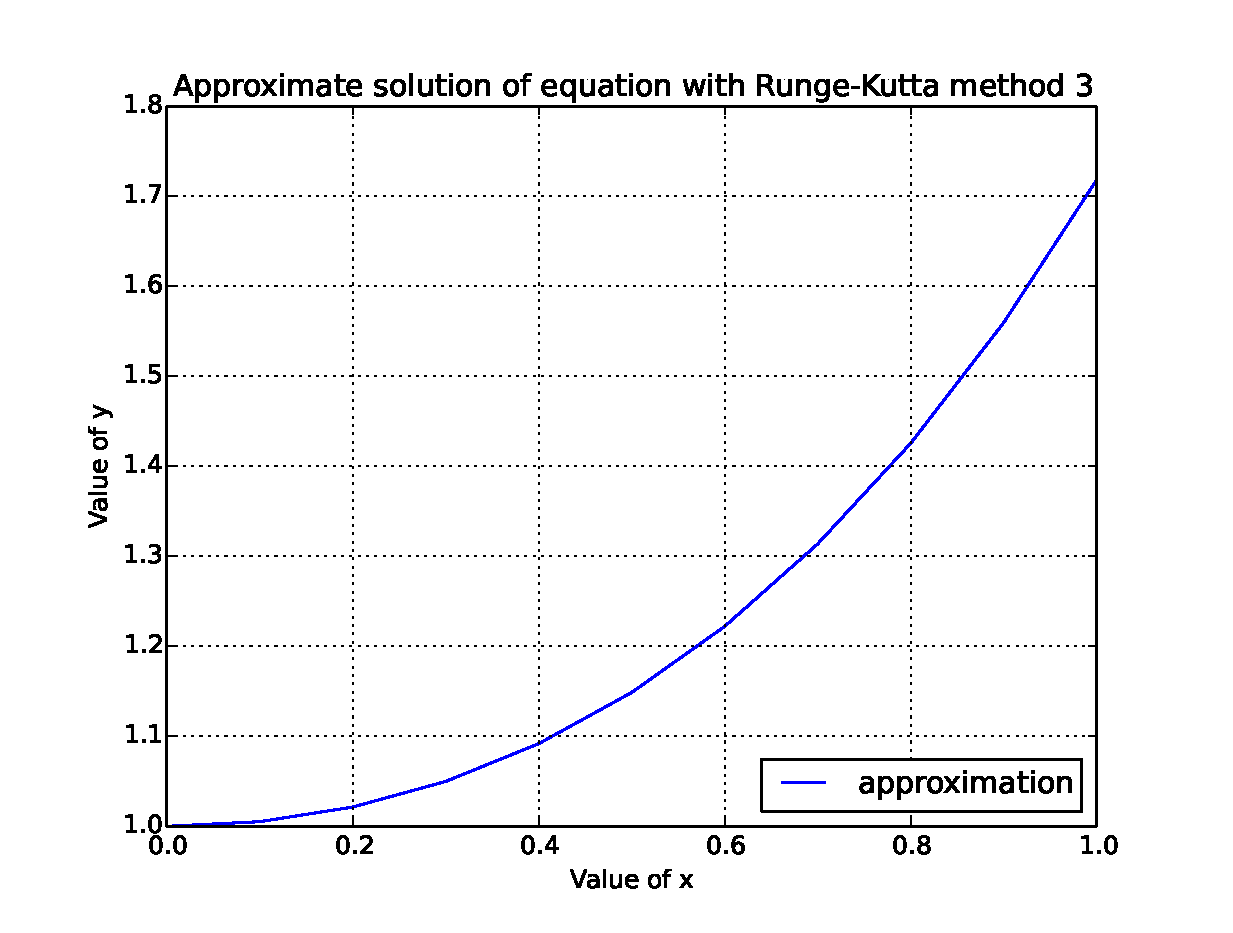
\includegraphics[width=8cm]{3_2.eps}
\end{figure}
\section{Solve $y'=(y^2-y)/x^2$ using Euler method and Runge-Kutta 4 method}
Let's try to approximate the value of the function in the interval [0.1, 1.0] with 10 points (if we start with 0 it will give division by zero). Then $x_0 = 0.1, y_0 = 1.0, x_f = 0, n = 10$, and $h = (x_f-x_0 )/(n-1)=0.1$. Following is the table after filling out the values of $y(x_i)$:
\begin{center}
\begin{tabular}{ |c|c| } 
 \hline
 $x$ & $y$\\
\hline
 $0.0$ & $0.0$ \\ 
 $0.1$ & $0.0$ \\ 
 $0.2$ & $0.0$ \\
 $0.3$ & $0.0$\\
 $0.4$ & $0.0$\\
 $0.5$ & $0.0$\\
 $0.6$ & $0.0$\\
 $0.7$ & $0.0$\\
 $0.8$ & $0.0$\\
 $0.9$ & $0.0$\\
 $1.0$ & $0.0$ \\
 \hline
\end{tabular}
\end{center}
If we try to plot the graph of this function result will be as follows:
\begin{figure}[h]
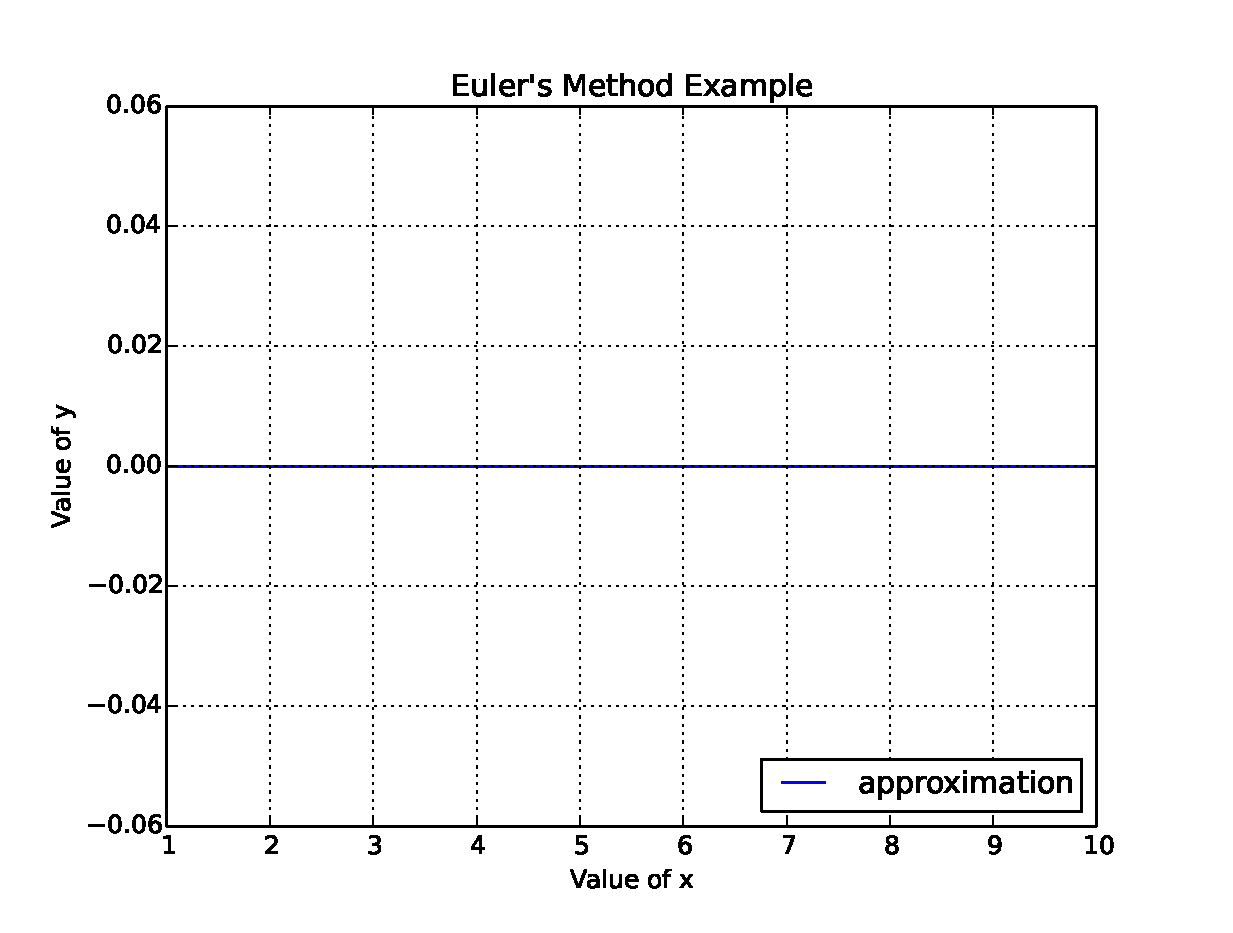
\includegraphics[width=8cm]{4_1.eps}
\end{figure}\\
Both methods give the same solution.
\section{Solve $y'=(1+y)/tan{x}$ using Modified Euler method 1 and Runge-Kutta method 4}
\subsection{Solution using Modified Euler method 1}
Let's try to approximate the value of the function in the interval [1.0, 10.0] with 10 points. Then $x_0 = 1.0, y_0 = 1.0, x_f = 10.0, n = 10$, and $h = (x_f-x_0 )/(n-1)=0.9$. Following is the table after filling out the values of $y(x_i)$:
\begin{center}
\begin{tabular}{ |c|c| } 
 \hline
 $x$ & $y$\\
\hline
$1.0$ & $1.0000000000000000$\\
$1.9$ & $1.0927286877177949$\\
$2.8$ & $-1.0633684619181731$\\
$3.7$ & $-0.9132600104639936$\\
$4.6$ & $-0.8400285429342458$\\
$5.5$ & $-0.9115549541314385$\\
$6.4$ & $-0.9189695157150598$\\
$7.3$ & $-0.4126897959522442$\\
$8.2$ & $-0.3975307758698257$\\
$9.1$ & $-1.0392086151305469$\\
$10.0$ & $-0.9412789357986875$\\
 \hline
\end{tabular}
\end{center}

If we try to plot the graph of this function result will be as follows:
\begin{figure}[h]
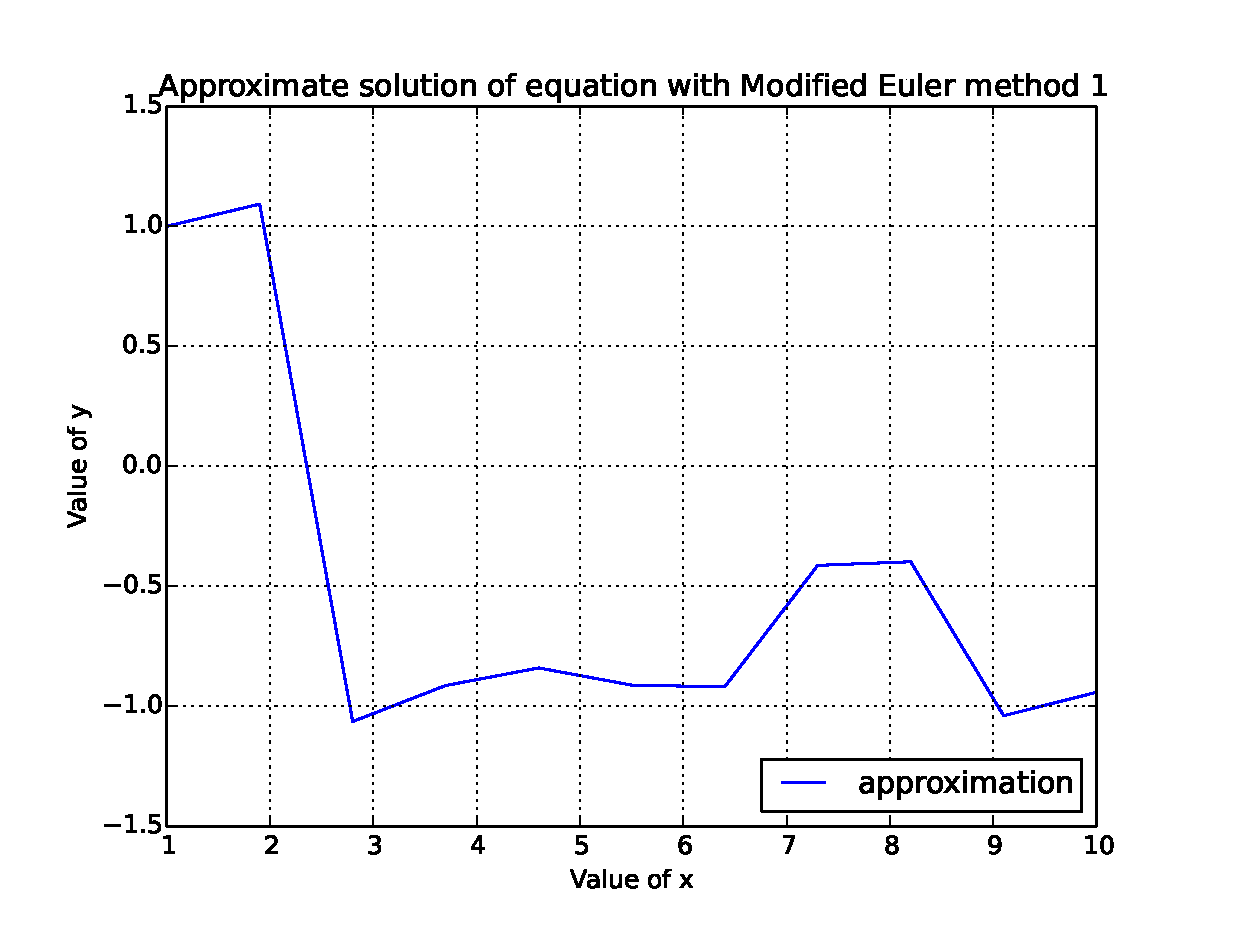
\includegraphics[width=8cm]{5_1.eps}
\end{figure}
\subsection{Solution using Runge-Kutta method 4}
I will be using the same interval as was above and we get the following values:
\begin{center}
\begin{tabular}{ |c|c| } 
 \hline
 $x$ & $y$\\
\hline
$1.0$ & $1.0000000000000000$\\
$1.9$ & $1.2499889202642265$\\
$2.8$ & $-0.2682690087484034$\\
$3.7$ & $-1.2796185692468598$\\
$4.6$ & $-1.5251095569943645$\\
$5.5$ & $-1.3714977166209588$\\
$6.4$ & $-1.1663710130927201$\\
$7.3$ & $-2.2165022273451749$\\
$8.2$ & $-2.3461039207834338$\\
$9.1$ & $-1.4133945810421138$\\
$10.0$ & $-0.6546702603992544$\\
 \hline
\end{tabular}
\end{center}
If we try to plot the graph of this function result will be as follows:
\begin{figure}[h]
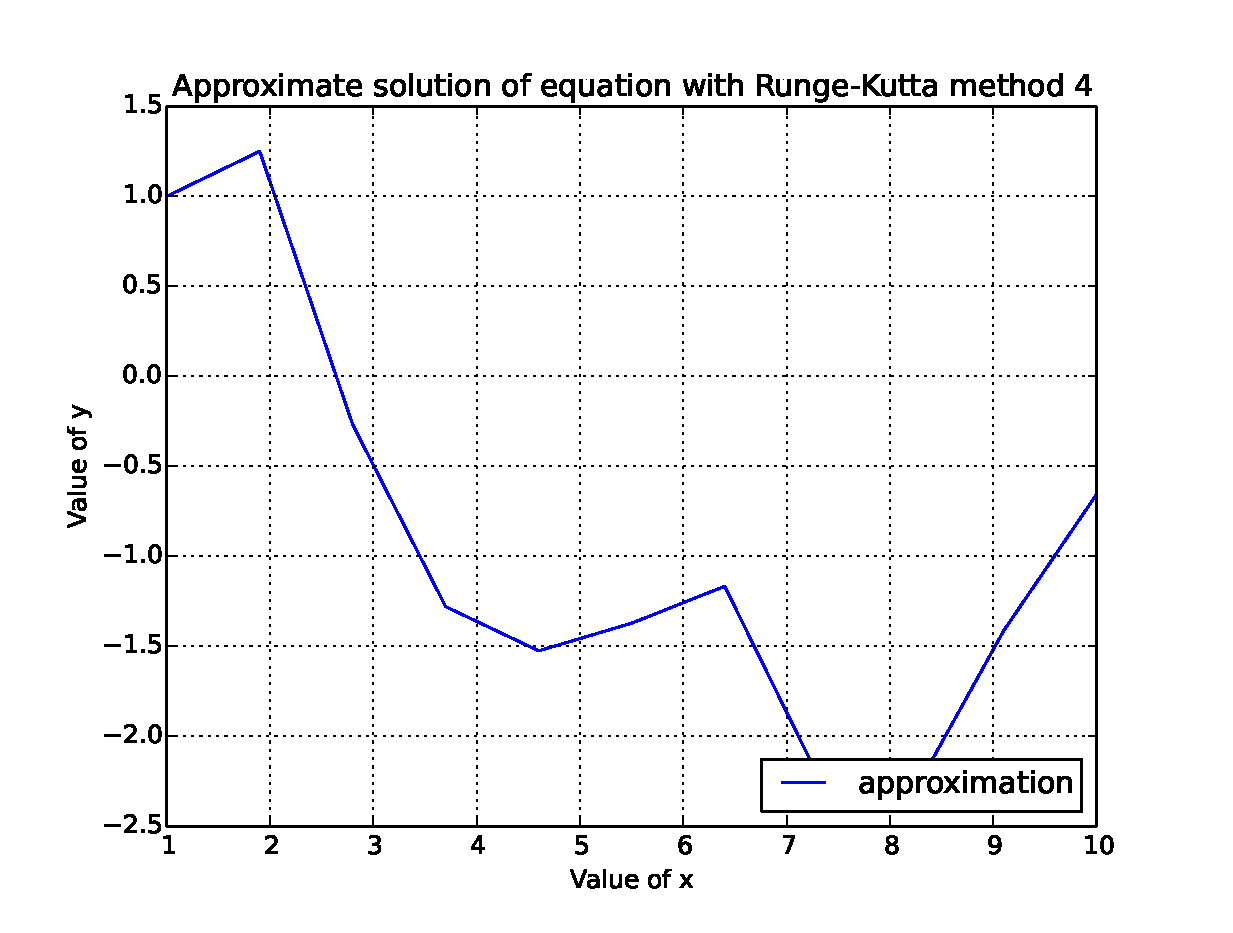
\includegraphics[width=8cm]{5_2.eps}
\end{figure}
\medskip

\begin{thebibliography}{9}
\bibitem{rosettacode} Rosetta Code Link, \\\texttt{https://rosettacode.org/wiki/Runge-Kutta-method}
\bibitem{euler} Euler Method PDF, \\\texttt{https://sites.math.washington.edu/~wcasper/math307-win16/review/euler-method/euler-method.pdf}
\bibitem{connor} Numerical Solutions to ODEs, \\\texttt{http://connor-johnson.com/2014/02/21/numerical-solutions-to-odes/}
\end{thebibliography}

\end{document}
